%!TEX root = ../template.tex
%%%%%%%%%%%%%%%%%%%%%%%%%%%%%%%%%%%%%%%%%%%%%%%%%%%%%%%%%%%%%%%%%%%%
%% chapter2.tex
%% NOVA thesis document file
%%
%% Chapter with the template manual
%%%%%%%%%%%%%%%%%%%%%%%%%%%%%%%%%%%%%%%%%%%%%%%%%%%%%%%%%%%%%%%%%%%%
\chapter{Related Work}
\label{cha:related_work}
Since the users are a fundamental component of the study, their relationship with data and what are their expectations of these query systems will be discussed. Moreover, a set of technologies and techniques will be described and compared. This information can turn to be useful to explore solution, and understand different points of view to manage problems, regarding the project scope. 

\section{Query Conceptual Models}
\label{sec:query_conceptual_models}
The perception of the user's conceptual model is important to understand how the user reason while interacting with the system the perform the intended actions. A query is built to gather data. To transmit what is the intended data, the user needs to think about how it could express the data required in the query. The understanding of the user's conceptual model could be useful to remove the existing gap between what the user wants to query from the database and what system register that the user wants to retrieve.

Some studies have analyzed this reasoning process of the users when they were writing queries. Siau \textit{et al.} \cite{effectsOfQueryComplexityAndLearningOnNoviceUserQueryPerformance} have referred that "The semantics communicated through the interface can be classified according to abstraction levels, such as the conceptual and logical levels". Also, there is one more level, the physical level, where is considered the system details, such as physical storage and access structures. Since the physical level is low level, usually, the conceptual and logical levels are most used. The logical level takes into account abstract structures for data and operations, and the conceptual level uses real-world objects and concepts to communicate. Through an empirical method of evaluation, the conceptual level has revealed a higher accuracy. Also, this abstraction level makes the users more confident in their answers than the physical level or logical levels. Moreover, the time that users need to design the queries is reduced using conceptual levels \cite{effectsOfQueryComplexityAndLearningOnNoviceUserQueryPerformance}.

Reisner \cite{humanFactorStudiesOfDatabaseQueryLanguages} provided a model of query writing from the reading of the query intention in an English statement to the query writing in \gls{SQL} (Figure \ref{fig:reisner_model}). After understanding what data is required, the user applies two parallel steps. In the \textbf{Template Generation} phase, the user formulates a template identifying the \gls{SQL} keywords necessary, such as SELECT, FROM, and WHERE. In the other step, called \textbf{Lexical Transformation}, the user identifies the name of the tables and columns involved. Finally, the results of these two steps are combined in the last step, denominated \textbf{Insertion}, in order to produce the final query \cite{humanFactorStudiesOfDatabaseQueryLanguages}. The recall of table and column names represents a significant use of long-term memory, being a concern that should be taken into account \cite{userErrorsInDatabaseQueryComposition}.

In the same field, Ogden \cite{implicationsOfACognitiveModelOfDatabaseQuery} presented a three-stage cognitive model of the query process (Figure \ref{fig:ogden_model}):

\begin{enumerate}
  \item \textbf{Query Formulation}: according to the existing data, the user specifies, in natural language, what data is required;
  \item \textbf{Query Translation}: regarding the existing data model, the operations and relations necessary are defined, in order to adapt the natural language request to the pragmatics of the intended query;
  \item \textbf{Query Writing}: the information of the previous steps is used to built the query, using the syntactic and the semantics of the query language.
\end{enumerate}

Comparing the two previous models, the Lexical Transformation phase is present in the Query Translation phase of the latter model, as well as, Template Generation and insertion are part of the Query Writing phase \cite{anEvaluationOfNoviceEndUserComputingPerformance}. Moreover, although the query writing and comprehension are the focus of this work, it was verified in a comparison between three different models (relational model, extended-entity-relationship model, and object-oriented model) that the data model influence the query writing and comprehension \cite{anEvaluationOfNoviceEndUserComputingPerformance}.

\begin{figure}[tb]
  \centering
  \subcaptionbox{Reisner Model\label{fig:reisner_model} (adapted: Reisner \cite{humanFactorStudiesOfDatabaseQueryLanguages})} %
    {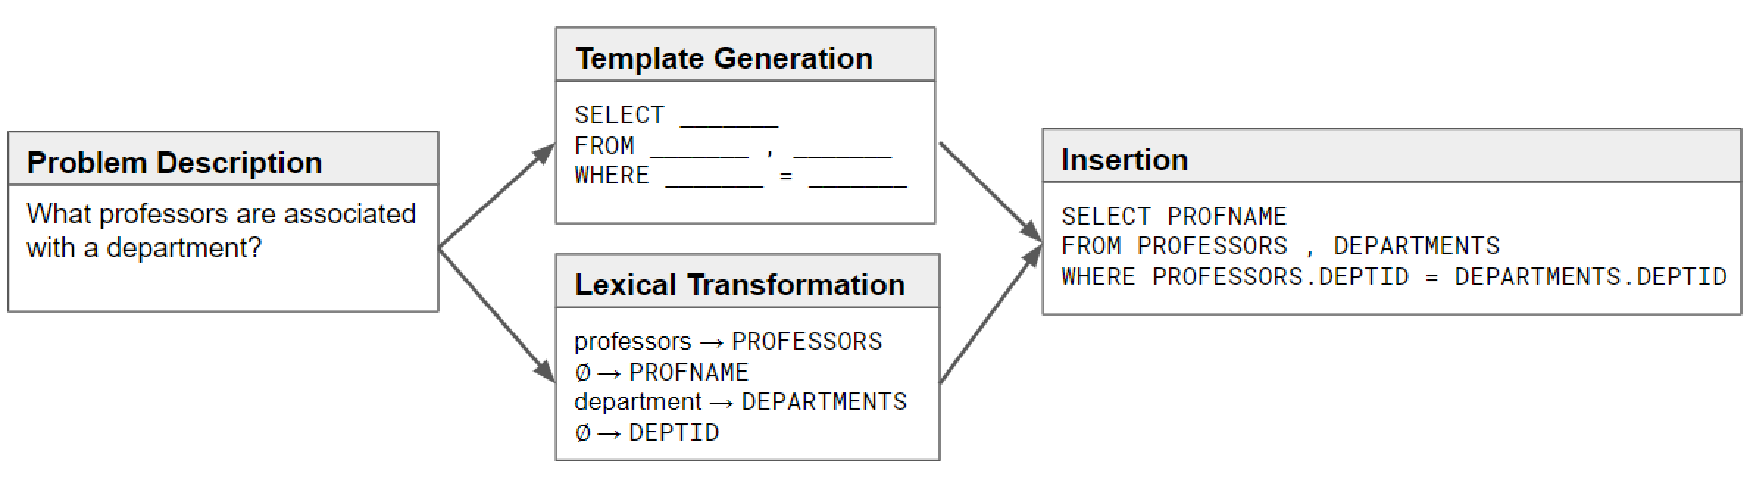
\includegraphics[width=0.9\linewidth]{reisner-model}}%
    \\
  \subcaptionbox{Ogden Model \label{fig:ogden_model} (adapted: Ogden \cite{implicationsOfACognitiveModelOfDatabaseQuery})}%
    {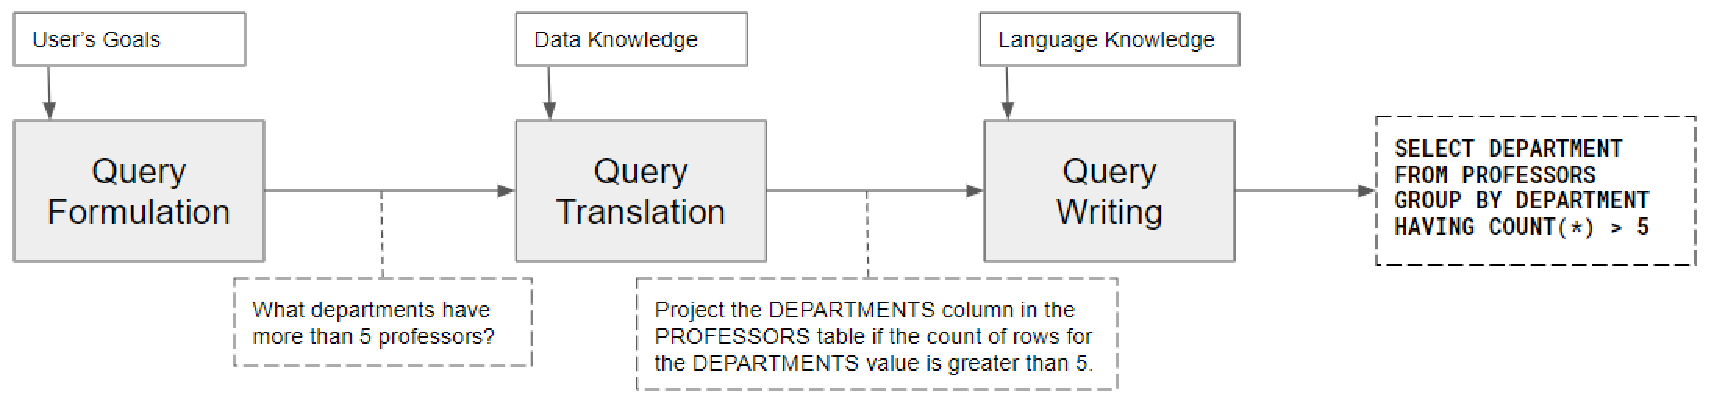
\includegraphics[width=0.9\linewidth]{ogden-model}}%
\caption{Models of Query Writing Process.}
  \label{fig:models_of_query_writing_process}
\end{figure}

The query comprehension is one of the important concerns of this work, since it is important to consider if the query representation, no matter if it is visual or textual, indicates clearly what data will be gathered. %TODO: pode ser importante dar exemplos da importancia da comprehension (e.g., para quem vai ler; se o escritor foi diferente do leitor, etc.) 
Chan \textit{et al.} \cite{anEvaluationOfNoviceEndUserComputingPerformance} have postulated that the query comprehension could be covered by the reverse of the stages included in the Ogden Model. First, the user should identify the data structure and operations, to translate them, in the next step, to the natural language. After this, the user needs to read and understand what data gathering is intended. Moreover, in this evaluation, it was concluded that although data modeling influence query writing, it does not influence the query comprehension. The explanation is provided by the authors: "Both query writing and comprehension require an understanding of the query language syntax. This is a component not needed in the data modeling task."

The experience with the data involved is another factor that influences the query comprehension. If novice users do not understand the data involved, they cannot validate if the query result is correct. This situation was analyzed by Robb \textit{et al.} \cite{improvingNewUsersQueryPerformance} that were distinguished the query process between new users and experienced users (Figure \ref{fig:ex_ante_expectations}). Besides, they concluded that if the novice users were alerted to the details of the data queried, the query effectiveness will increase.

\begin{figure}[tb]
  \centering
    {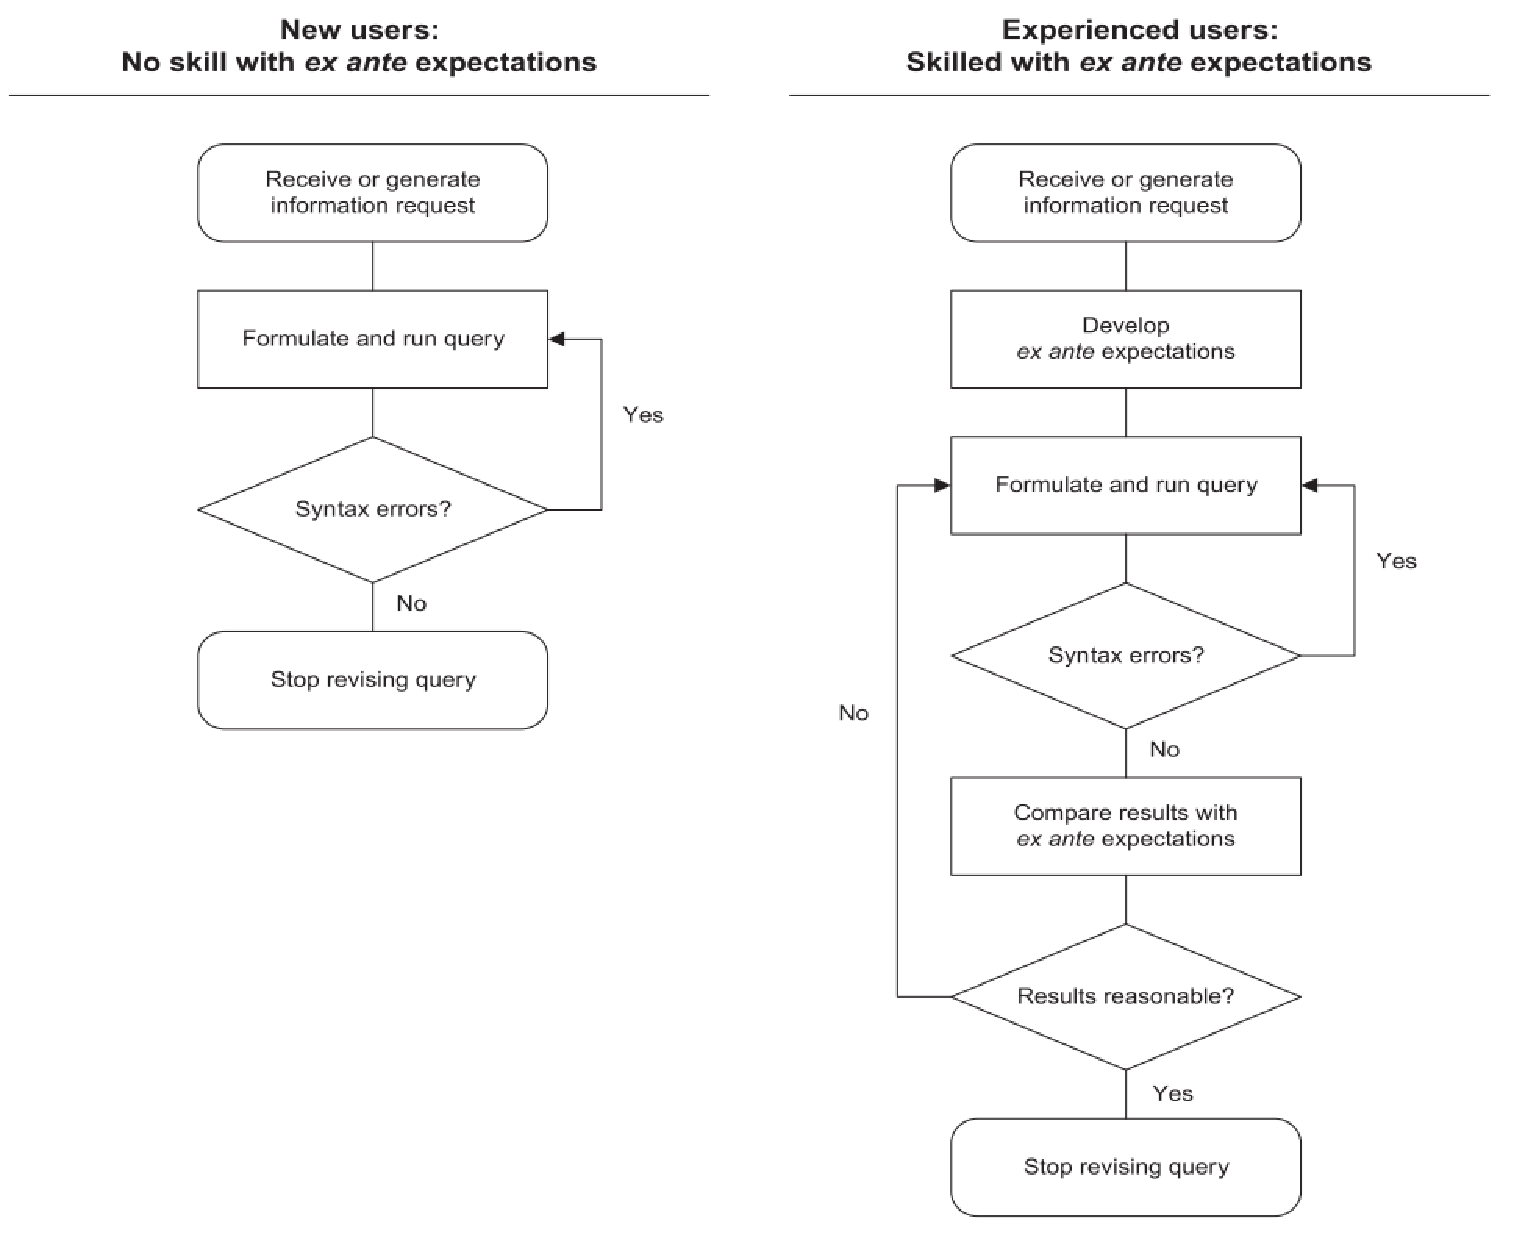
\includegraphics[width=1.0\linewidth]{ex-ante-expectations}}%
\caption{New and experienced users’ query processes (source: Robb \textit{et al.} \cite{improvingNewUsersQueryPerformance}).}
  \label{fig:ex_ante_expectations}
\end{figure}


\section{Query Formulation Problems}
\label{sec:query_formulation_problems}
Since the goal of this work is the improvement of an interface that allows its user to build queries, it is important to summarize a set of significant problems that usually occur in query formulation. The problems that will be presented are related to \gls{SQL} queries. However, as the visual tool of this work aims to substitute some functionalities of \gls{SQL}, the comprehension of the interaction problems that exist in the textual language can be considered and mitigated in the development of the new interface. 

Lu et al. \cite{aSurveyOnUsageOfSQL} have evaluated the \gls{SQL} usage in a diverse population, which includes people of different enterprise areas with different levels of experience in the database systems domain. The authors concluded that the comprehension of the queries is difficult, as well as the logical errors are difficult to detect. Moreover, the joins and aggregation functions are the other problems pointed out.

The query errors could be syntactic or semantic. The \textbf{Syntactic Errors} are related to the grammar rules of the language and are detected by the compiler. Therefore, the impact of these errors is reduced since the user can see that the query is incorrect through the compiler alert. The \textbf{Semantic Errors} are a major concern because they occur when the returned information is not intended by the user, even if the query does not have compilation errors \cite{userErrorsInDatabaseQueryComposition}. These errors could affect the correctness of the results.

In \gls{SQL}, the join clauses are used when is necessary to merge data from different tables in one column in order to specify which data of each table will be considered. Several studies have demonstrated that the indication of the join clause is one of the most representative semantic errors \cite{studentsSemanticMistakesInWritingSevenDifferentTypesOfSQLQueries,aSurveyOnUsageOfSQL}. Smeller \cite{userErrorsInDatabaseQueryComposition} has studied what are the cognitive causes that lead the user to forget the join clauses:

\begin{itemize}
  \item \textbf{Working memory overload}: if the user needs to recall the table and column names, and the conditions necessary after the identification of the join's requirement, the required join clauses could be forgotten in this period;
  \item \textbf{Absence of the clue}: when the statement that explains what data is required do not present clues for the join necessity;
  \item \textbf{Procedural fixedness}: when a query that only extracts data from one table is reused for another that requires the join clauses but this join is forgotten;
  \item \textbf{Ignorance}:  when the user does not know how to merge the tables and specify the join clauses.
\end{itemize}

The cognitive causes of the problems are important to develop interfaces that could mitigate the existing problems in the query formulation. For instance, if the join clues are provided in the interface, the user does not need to remember them. This approach, which follows one of the usability heuristics presented by Nielsen \cite{usabilityEngineering}, minimizes the user memory load.

A study that evaluated novice programmers' semantic mistakes concluded also that omissions are the principal semantic error, mainly in the WHERE clause \cite{studentsSemanticMistakesInWritingSevenDifferentTypesOfSQLQueries}. Besides, the authors have referred also the problem of working memory overload: "This error may occur when the capacity of a student’s working memory is surpassed".

Another study has analyzed a large dataset of queries composed by university students enrolled in an introductory database course. However, this study is more extensive and includes a list of the principal errors committed by the students \cite{errorsAndComplicationsInSQLQueryFormulation}. Continuing the focus on the semantic errors, the authors have pointed out the following error categories: inconsistent expressions, inconsistent joins, joins omission, duplicate rows, redundant column outputs \cite{errorsAndComplicationsInSQLQueryFormulation}.

\section{Visual Query Composition}
\label{sec:visual_query_composition}

The interfaces to build queries resort to visual representations to communicate with the user. Catarci \textit{et al.} \cite{visualQuerySystemsForDatabases_aSurvey} presented an interesting classification according to the visual formalism which the interface is based on:

\begin{itemize}
    \item \textbf{Form-based}: based on forms, which can be seen as a rectangular grid of other components (subforms, groups of cells, a combination of cells, etc.) that group objects in a named collection regarding its structure. Forms and tables are similar,  but contrary to the tables, forms allow nesting. Thus, forms can be seen as a generalization of tables. In this approach, the relationships can be represented among cells, cells subsets, or even the overall set, providing to the user three information levels; %TODO: example of QBE 
    \item \textbf{Diagram-based}: usage of graphical representations, such as graphs, charts, and diagrams to better transmit the relationships among data. The aim is to use visual representations to help the understanding of the relationships between concepts which are represented by textual labels;
    \item \textbf{Icon-based}: as the opposite of the diagram-based, this type of interface tries to facilitate the understanding of the concepts instead of relationships. So, Icons are used, which are visual segmented objects to transmit a message or information, using analogies and metaphors with the real-world objects, or even conventions that are used to express no tangible objects, as computer processes;
    \item \textbf{Hybrid}: these approaches can combine the previous visual formalisms in order to select the best combination of advantages to the application usage domain.
\end{itemize}

In order to compare different interfaces, it is essential to analyze what a query language has to support to build the query. Accordingly, Table \ref{tab:query_language_requisites} presents the query creation required specifications, comparing them with the respective indication in \gls{SQL}.

\begin{table}[tb]
	\caption{Query Language Requisites}
	\label{tab:query_language_requisites}
\centering
\resizebox{\textwidth}{!}{
\begin{tabular}{|
    >{\columncolor[HTML]{EFEFEF}}l |l|l|}
    \hline
    \cellcolor[HTML]{C0C0C0}{\color[HTML]{333333} \textbf{Specification}} & \cellcolor[HTML]{C0C0C0}{\color[HTML]{333333} \textbf{Description}}                                                                                               & \cellcolor[HTML]{C0C0C0}{\color[HTML]{333333} \textbf{SQL Indication}}                                                                   \\ \hline
    \textbf{Data Source}                                                  & \begin{tabular}[c]{@{}l@{}}Entities and attributes which \\ will be presented in the query\end{tabular}                                                           & \begin{tabular}[c]{@{}l@{}}Using SELECT and \\ FROM statements\end{tabular}                                                              \\ \hline
    \textbf{Merge Type}                                                   & \begin{tabular}[c]{@{}l@{}}Define how will be merged \\ attributes of different entities\end{tabular}                                                             & Using JOIN clauses                                                                                                                       \\ \hline
    \textbf{Filtering Criteria}                                           & \begin{tabular}[c]{@{}l@{}}Criteria that can be used to \\ filter records, presenting in the \\ result only those that fulfil a \\ set of conditions\end{tabular} & \begin{tabular}[c]{@{}l@{}}Using WHERE  or \\ HAVING clauses\end{tabular}                                                                            \\ \hline
    \textbf{Sorting Criteria}                                             & \begin{tabular}[c]{@{}l@{}}Define what are the criteria to \\ sort the records of the result\end{tabular}                                                         & \begin{tabular}[c]{@{}l@{}}Using ORDER BY \end{tabular}                                                                         \\ \hline
    \textbf{Aggregation Functons}                                         & \begin{tabular}[c]{@{}l@{}}Group a set of records by \\ comparison or using mathematical \\ functions\end{tabular}                                                & \begin{tabular}[c]{@{}l@{}}Using  GROUP BY \\ statements or SQL \\ functions, such as \\ MIN, MAX, \\ COUNT, AVG and \\ SUM\end{tabular} \\ \hline
    \textbf{Calculated Attributes}                                        & \begin{tabular}[c]{@{}l@{}}Attributes added, based on \\ existing ones\end{tabular}                                                                               & \begin{tabular}[c]{@{}l@{}}Using SELECT \\ statement\end{tabular}                                                                        \\ \hline
    \textbf{Distinct Values}                                              & \begin{tabular}[c]{@{}l@{}}If only different values will be \\ considered in the result \\ (removing duplicated values)\end{tabular}                              & \begin{tabular}[c]{@{}l@{}}Using SELECT \\ DISTINCT statement\end{tabular}                                                               \\ \hline
    \textbf{Unions}                                                       & \begin{tabular}[c]{@{}l@{}}Combine the result of two \\ different queries\end{tabular}                                                                            & \begin{tabular}[c]{@{}l@{}}Using UNION \\ operator\end{tabular}                                                                          \\ \hline
    \textbf{Subqueries}                                                   & \begin{tabular}[c]{@{}l@{}}Defining a query that uses \\ other queries, for example, \\ to filter the result\end{tabular}                                         & \begin{tabular}[c]{@{}l@{}}Nesting SELECT \\ statements\end{tabular}                                                                     \\ \hline
    \end{tabular}
}
\end{table}

Nevertheless, there are two relevant aspects, according to the last requisites presented: the interaction process to indicate the query specifications, the overview of what data wants to be retrieved using the current query. Both are fundamental since a good visual query language aims to simplify not only, the query formulation process but also, the query readability, promoting an efficient and effective recognition of what are the desired data.

\textbf{Data Source:}

Chartio \cite{chartio} has two components to query databases visually: using the Data Explorer \cite{chartioDataExplorer} or using the new Visual SQL \cite{chartioVisualSQL}. Regarding the data source specification, these two systems use different strategies to select and present the entities and attributes related to the query. In the Data Explorer, the user can expand the items of a list of tables in a scrollable and searchable tree view, which is pinned in one side of the window, to choose the desired attributes. This system divides the attributes into two different types: Measures and Dimensions. Usually, measure refers to quantitative data and dimensions to categorical data. So, to insert the attributes in the query, users can drag and drop the required attributes to the form-based interface that contains the Measures, Dimensions, and Filters of the query (Figure \ref{fig:chartioDataExplorer}) \cite{chartioDataExplorer}. 

On the other hand, the new component of Chartio, Visual SQL provides a different interface to select the data sources. Contrary to the previous approach, in this interface, there is no fixed list to choose the attributes. In this way, there is only a search text component that is activated when the user clicks on “add column” action. When this action occurs, a pop-up style component that has a list, similar to the referred above, where it is possible to preview some data entries of the table, is presented (Figure \ref{fig:chartioVisualSQL}) \cite{chartioVisualSQL}. 

In the systems referred above the columns are added one by one sequentially, but other systems have different methods to select the table’s columns. For example, in Tableau Prep \cite{tableauPrep} there is a checkbox list to chose the intended attributes (Figure \ref{fig:tableauPrep}), and in Microsoft Power BI \cite{powerBI} the table is chosen using a list, and all its attributes are added automatically. Also, users can remove, the columns not desired afterwards \cite{tableauPrepHelpWhatsNew,powerBIShapeAndCombineData}.

Other systems, as Devart dbForge Query Builder \cite{dbForgeQueryBuilder}, uses a diagram-based interface to select the entities and attributes of the query. In this system, the user can drag and drop the desired tables to the diagram area, and select through checkboxes the intended attributes, that are presented in the database schema diagram (Figure \ref{fig:devartDbForge}).


\begin{figure}[tb]
    \centering
    \subcaptionbox{Chartio Data Explorer\label{fig:chartioDataExplorer} (source: Chartio\cite{chartioDataExplorer})}%
      {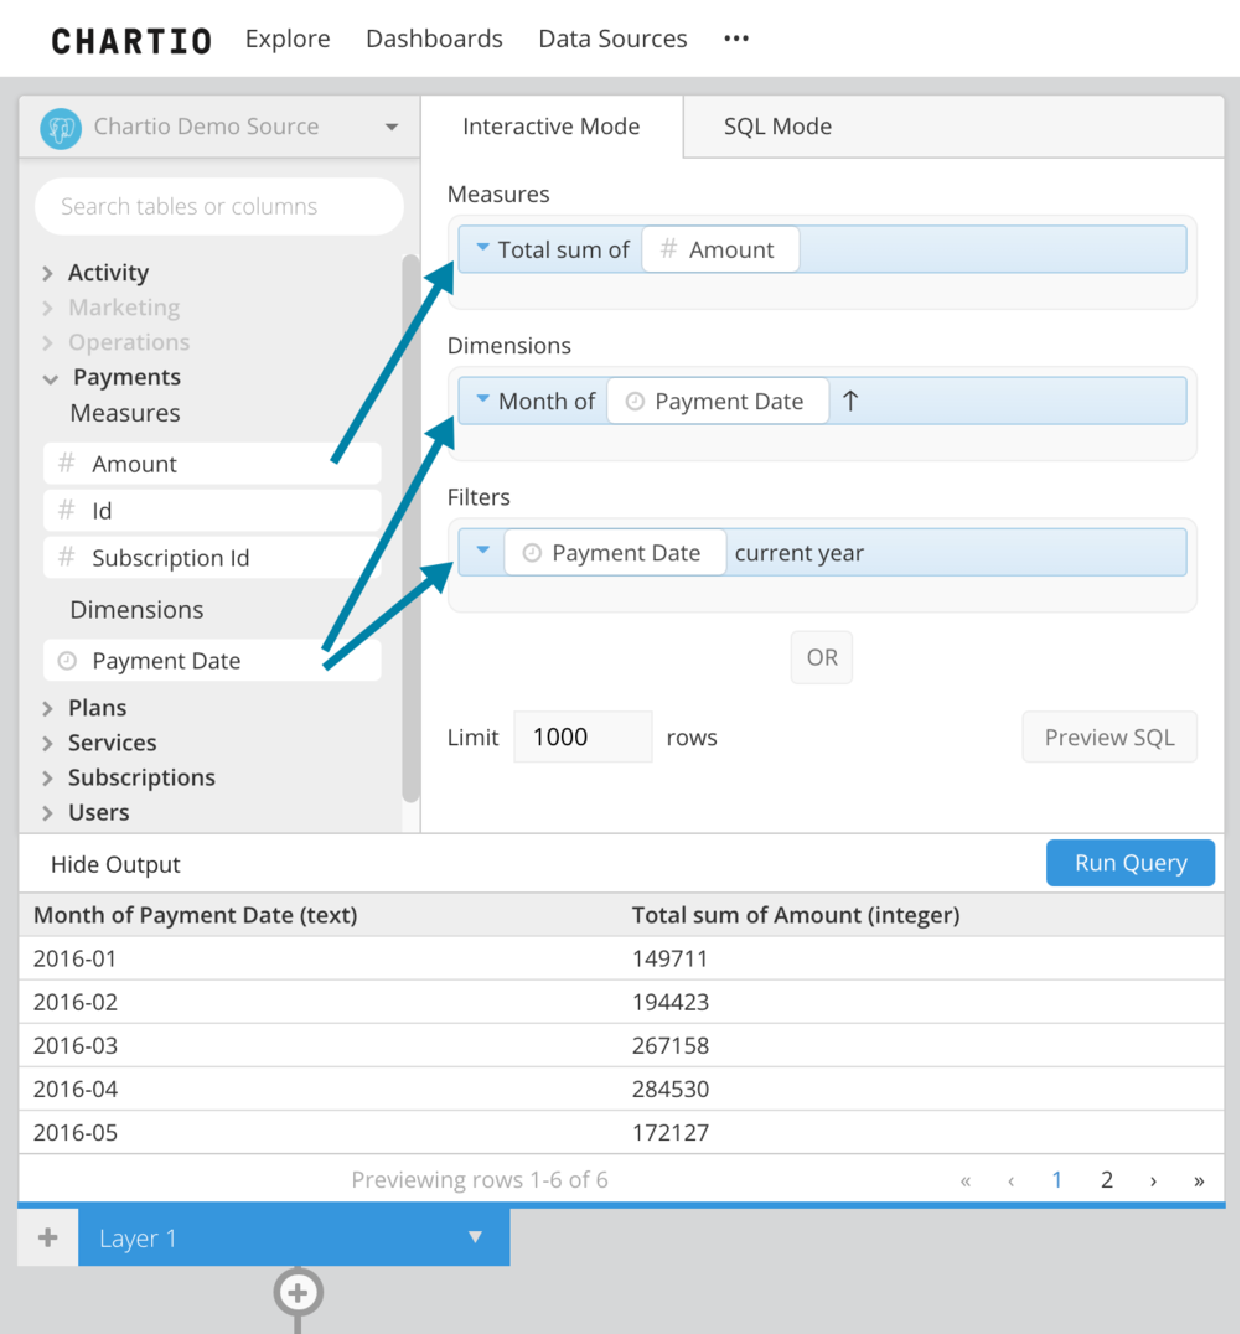
\includegraphics[width=0.5\linewidth]{chartio-data-explorer-data-source}}%
    \subcaptionbox{Chartio Visual SQL\label{fig:chartioVisualSQL} (source: Chartio \cite{chartioVisualSQL})}%
      {\includegraphics[width=0.5\linewidth]{chartio-visual-SQL-data-source}}%
      \\
    \subcaptionbox{Tableau Prep\label{fig:tableauPrep} (source: Tableau \cite{tableauPrepHelpWhatsNew})}%
    {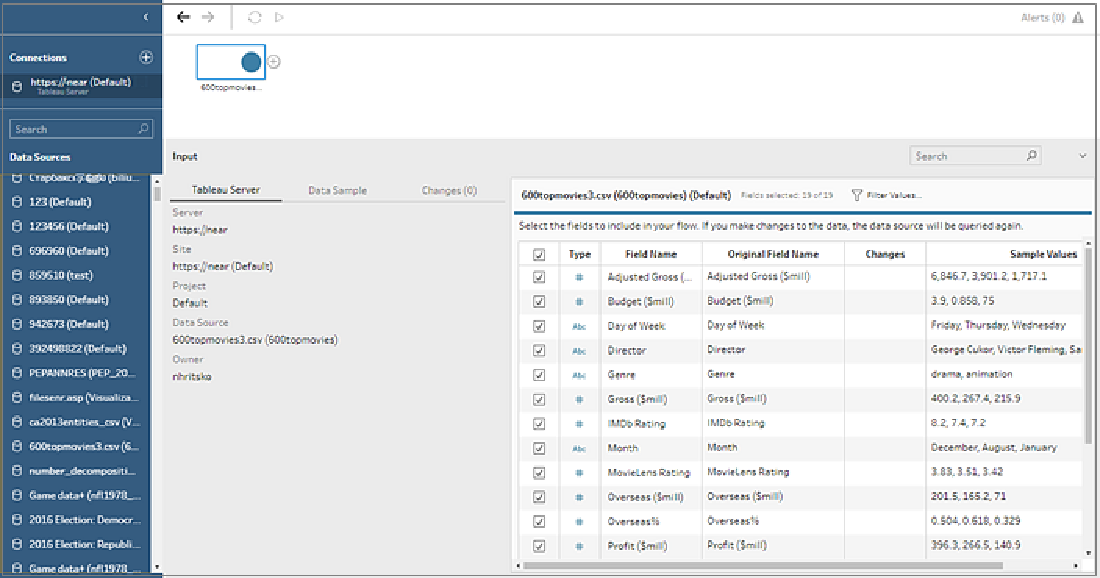
\includegraphics[width=0.5\linewidth]{tableau-data-source}}%
  \subcaptionbox{Devart dbForge Query Builder\label{fig:devartDbForge} (source: Devart \cite{dbForgeQueryBuilder})}%
    {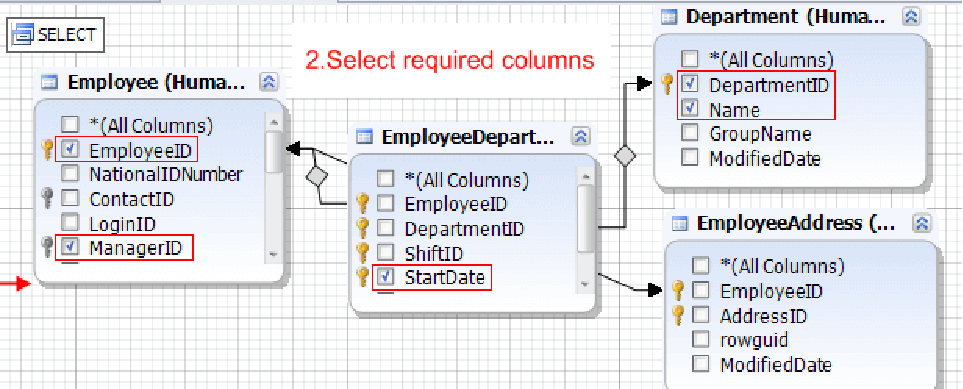
\includegraphics[width=0.5\linewidth]{dbforge-data-source}}%
  \caption{Different approaches to select the entities of the query.}
    \label{fig:approaches_select_data_sources}
  \end{figure}

\textbf{Merge Type:}



Merges are used when it is necessary to extract data from different tables, so it is necessary to establish what is the join kind to merge the data. Therefore, the interface needs to adopt an interaction and representation technique to specify it. To define a join in Devart dbForge Query Builder \cite{dbForgeQueryBuilder}, the user can only select the attributes’ checkboxes of the different tables and the system generates an inner join automatically. In this system, there are buttons on the toolbar to select all rows of one table, of another, or both, allowing to perform left, right and outer joins respectively \cite{dbForgeMakingJoinsBetweenTables}.
  
Another approach used by some systems, such as Chartio Data Explorer \cite{chartioDataExplorer} and Microsoft Power BI \cite{powerBI}, is a form-based interface to insert a join. In the former, two queries can be merged clicking on a button to popup a form that can be used to select the merge type and the first columns that will be merged using dropdowns \cite{chartioDataExplorer} (Figure \ref{fig:chartioDataExplorerJoin}). Also, if there are null values on the merge related columns, there is an option to include or not the null values match rows \cite{chartioJoiningDataAcrossDatabases}. Similarly, the latter provides a button to merge queries that opens a modal where the attributes that will be used on the merge (viewing also a table preview) and the join kind can be chosen, using a dropdown \cite{powerBIShapeAndCombineData} (Figure \ref{fig:powerBIJoin}).
  
Tableau Prep \cite{tableauPrep} provides two options to start a join between two tables: clicking on a "add join" hover button above the table visual representation with the suggestion of related tables, or merge the visual representation of two tables using a drag and drop action. After this selection, the inner join type is selected automatically by the system according to the tables' relationship \cite{tableauAggregateJoinOrUnionData,tableauAddMoreDataInTheInputStep}. However, the user can configure the join in a dedicated section (Figure \ref{fig:tableauJoinPanel}) where it is possible to define the join type using a Venn Diagram, to manage the join clauses using dropdown lists to select the fields, including also some join clause recommendations based on the database schema. Moreover, a summary of the join result that contains counters with the values included and excluded by each table, in a visual way using diagrams is provided. Finally, a list of the values included and excluded, where the red values represent the values excluded is presented, as well as a preview of the join result \cite{tableauAggregateJoinOrUnionData}.

\begin{figure}[tb]
    \centering
    \subcaptionbox{Chartio Data Explorer\label{fig:chartioDataExplorerJoin} (source: Chartio \cite{chartioDataExplorer})}%
      {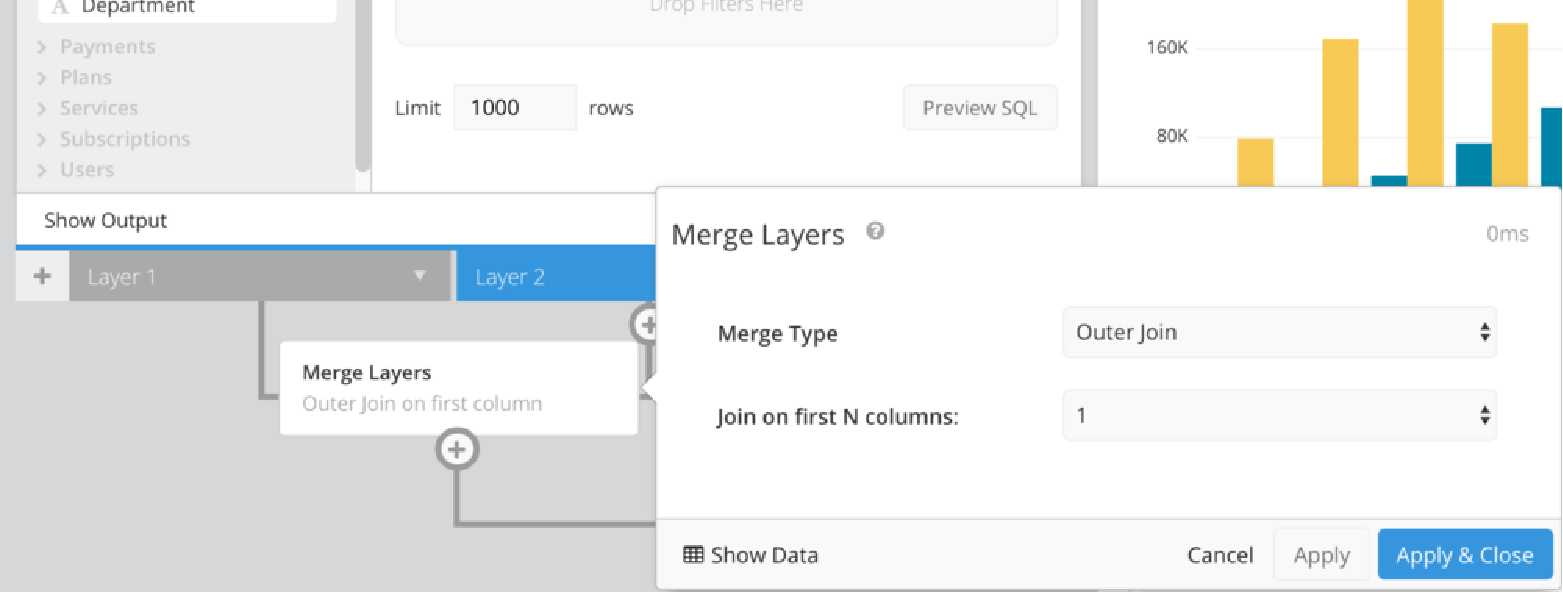
\includegraphics[width=0.5\linewidth]{chartio-data-explorer-join}}%
    \subcaptionbox{Microsoft Power BI\label{fig:powerBIJoin} (source: Microsoft \cite{powerBIShapeAndCombineData})}%
    {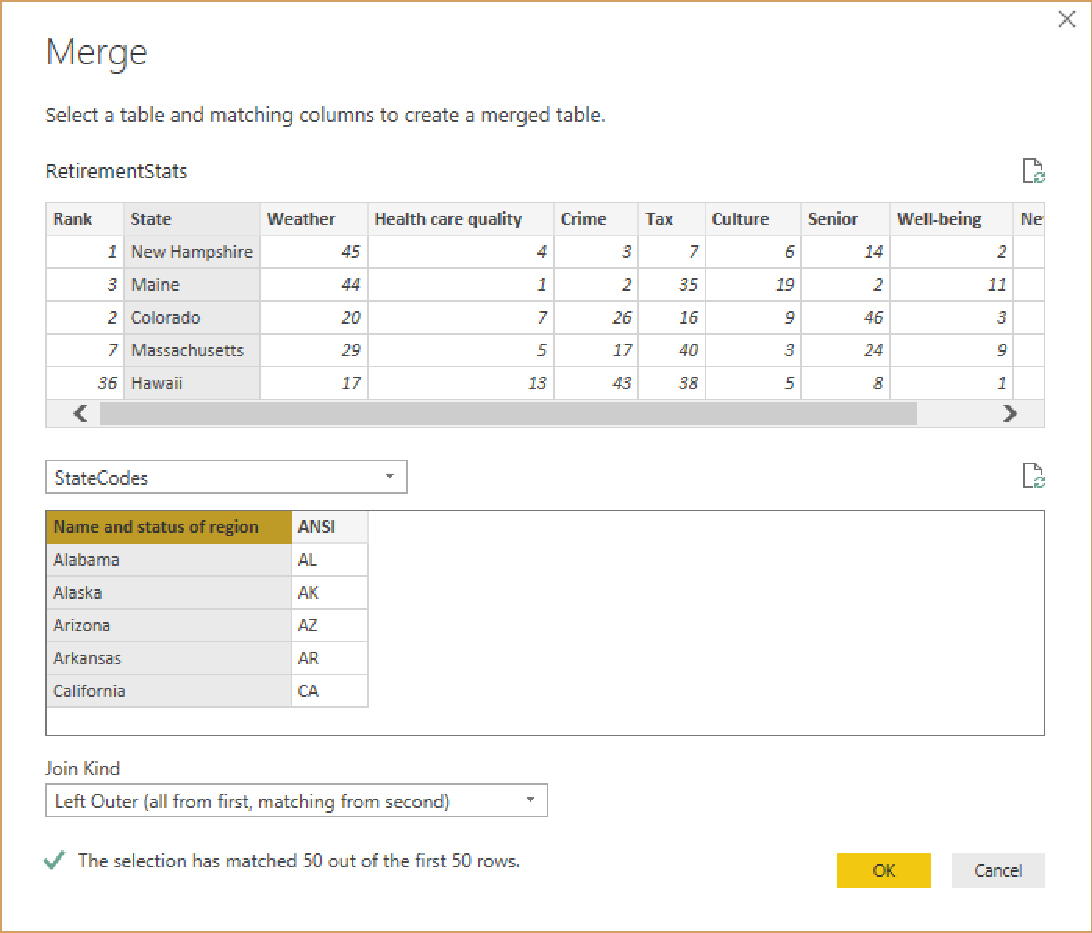
\includegraphics[width=0.5\linewidth]{power-bi-join}}%
    \\
    \subcaptionbox{Tableau Prep\label{fig:tableauJoinPanel} (source: Tableau \cite{tableauJoinImage})}%
      {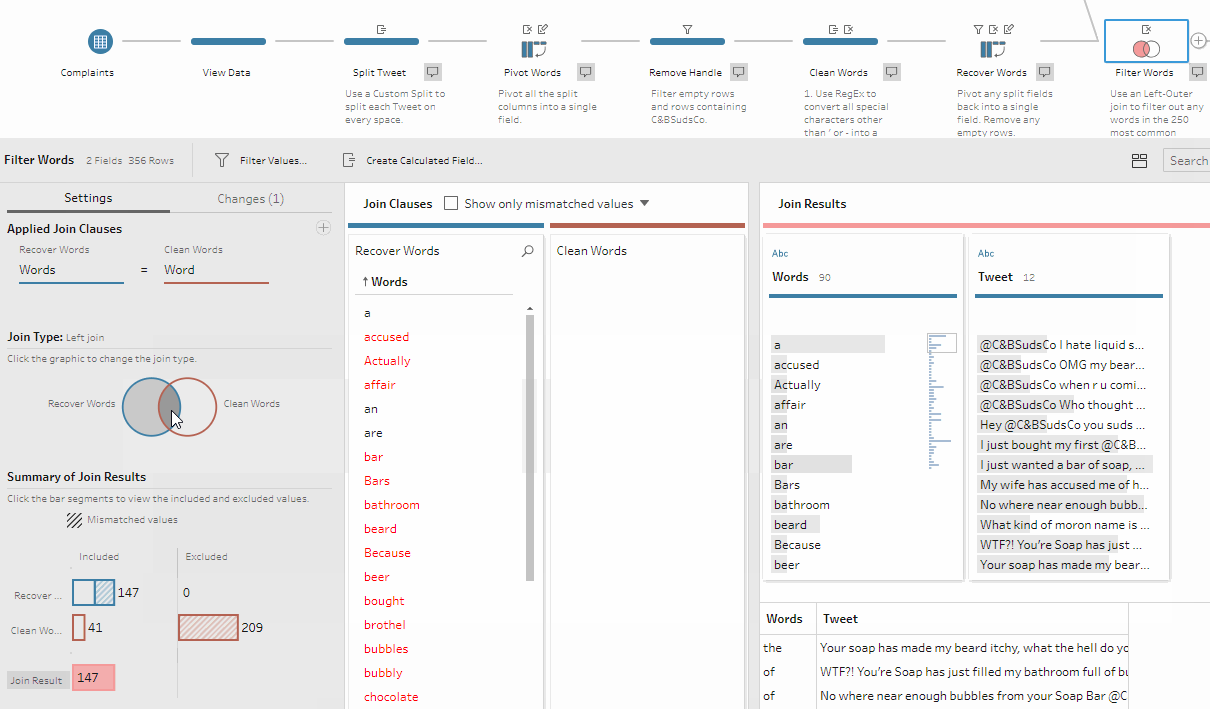
\includegraphics[width=1.0\linewidth]{tableau-join}}%
  \caption{Data merging approaches.}
    \label{fig:approaches_select_data_sources}
\end{figure}

\textbf{Filtering Criteria}: 

To represent and manage the filtering criteria of the queries, usually it is used text to indicate the logical conditions. However, some systems are trying to optimize the usability, helping the user in the specification process through some autocompletes. These diminish the necessity to remember all the syntax and the name of the functions. 
Besides, other systems present the logical conditions using a more structured layout, although keeping resorting in a textual representation. An example is Devart dbForge Query Builder \cite{dbForgeQueryBuilder} that represents the WHERE and HAVING clauses in a tree where the user can organize the conditions into groups \cite{dbForgeBuildingWhereOrHavingClause}.

Furthermore, some query systems also allow the user to view the query result, providing a shortcut in the column's name to insert filters. So, the user can change the query while is viewing the results. In this way, the user can apply a filter and view its effect almost immediately. Power BI Query Editor \cite{powerBI} is an example of a system that uses this approach.

Different interfaces can be used to select filters regarding the field data type. The advantages of the graphical interfaces could support the filtering criteria definition. For example, if a filter is applied to constraint dates, then a date input box with a visual calendar can be useful to simplify the date typing. In this way, some software, such as Chartio Visual SQL \cite{chartioVisualSQL} and Chartio Data Explorer \cite{chartioDataExplorer}, not only helps in the data typing but also provide dropdown lists that contain operators that can be applied to the referred data type (e.g. less than, contains, like, etc)  to helps the user in the boolean operator specification \cite{chartioDataExplorer,visualSqlActions}.

Tableau Prep \cite{tableauPrep} follows this more strictly, distinguishing between data types when filtering criteria are indicated. It provides different forms depending on the data type. The main difference of this system is that not only provides a more diversity of controls, as integrating range selectors, radio button, and the option to include or exclude fields through an action accessible near its value, but also gives to the user the option to use a calculation form where the interaction style is more textually and more extensible \cite{tableauFilterYourData}.

\textbf{Sorting Criteria}: 

Usually, in the actual \glspl{VQI}, the sorting criteria could be indicated in two ways: a right-click action on the column header of the table that represents the query result, or using a form-based interface to define the sort criteria of each entity. Devart dbForge Query Editor \cite{dbForgeQueryBuilder} is a pure example of the first approach \cite{dbForgeSortingData}. Chartio Data Explorer \cite{chartioDataExplorer} adopts the second approach, providing a pop-up form to apply sorting criteria to the query. The user can use this form to select the intended attributes and the criteria to apply \cite{chartioAdvancedSorting}. Moreover, Chartio Visual SQL \cite{chartioVisualSQL}, Tableau Prep \cite{tableauPrep}, and Microsoft Power BI \cite{powerBI} combines the previous solutions with the possibility to redefine the priority of the sorting criteria, through drag-and-drop actions \cite{visualSqlActions,tableauSortData,powerBIShapeAndCombineData}.

\textbf{Aggregation Functions}: 

In order to perform aggregations functions, such as MIN, MAX, COUNT, AVG, SUM, or GROUP BY, some systems provide these functionalities through interaction with the query result table. Devart dbForge Query Editor \cite{dbForgeQueryBuilder} provides this option to create an aggregation function. Moreover, in this editor exists another aggregation dedicated view which contains the aggregation functions in a tree view. In this view, users can group or ungroup the elements present in the window \cite{dbForgeGroupingDataInGrid}. Microsoft Power BI \cite{powerBI} allows also the users to add aggregations through the right-clicking on the column header, but in this case, it is open a form to enter the intended function and columns \cite{powerBICommonQueryTasks}. Chartio Visual SQL \cite{chartioVisualSQL} and Chartio Data Explorer \cite{chartioDataExplorer} presents a pop-up form where could be selected the columns and the aggregations intended \cite{chartioDataPipelineSteps}. Using a different interaction strategy, in Tableau Prep \cite{tableauPrep}, the user drag and drop the desired columns to a specific area that is divided into two: Grouped Fields and Aggregated Fields. The first is to add the \gls{SQL} corresponding GROUP BY, and the second to add the other aggregation functions, such as COUNT, MIN, MAX, AVG, and SUM.

\textbf{Other Specifications}: 

Regarding the option to add new calculated attributes, all the systems referred above allow inserting calculated attributes to the query, excepting the Devart dbForge Query Editor which does not support \cite{visualSqlActions,tableauCalculatedField,powerBICommonQueryTasks}.

The option to show only distinct values is provided in Tableau Prep \cite{tableauPrep}, Microsoft Power BI \cite{powerBI}, and Devart dbForge Query Editor \cite{dbForgeQueryBuilder}, through a button or a checkbox to does not see in the result the duplicated values. However, Chartio Visual SQL \cite{chartioVisualSQL} and Chartio Data Explorer \cite{chartioDataExplorer} does not support a specific interaction method to specify this. Nonetheless, the distinct effect can be applied, using the group by in all the columns of the query.

Some system provides visual options to build queries that contain UNIONs. For example, Chartio Visual SQL \cite{chartioVisualSQL} and Chartio Data Explorer \cite{chartioDataExplorer} provides this option in the same components of the joins. In these systems, when the user chooses the join type, the union is one of the join types available, although there is a different operation in \gls{SQL}. Tableau Prep \cite{tableauPrep} and Microsoft Power BI \cite{powerBI} present different options between the joins and unions, but the interface and the interaction strategies are similar \cite{tableauAggregateJoinOrUnionData,powerBIShapeAndCombineData}.

Moreover, a visual way to perform subqueries is provided by the diagrammatic-based interface of Devart dbForge Query Editor \cite{dbForgeQueryBuilder}, using tabs to alternate between the selected query. Links are used as assistants and shortcuts to view and change between the queries \cite{dbForgeSubqueriesOverview,dbForgeSubqueriesInFromClauses}.

\section{Discussion}
\label{sec:discussion}
The conceptual models of query writing presented in this chapter will be taken into account along the design of the solution since these are a good baseline to understand how users reason while are interacting with the system to achieve their goals. The system's tasks will be optimized according to the presented users' conceptual models presented, in order to reduce the semantic errors, as much as possible. Therefore, the most relevant semantic errors that occur using \gls{SQL} were presented. In the design of the solution, these errors are part of the problems to solve using a new user interface and \gls{UX}. As referred in section \ref{sec:query_formulation_problems}, the semantic errors will be the main concern since these could have a negative impact on the results. The syntactic errors also will be addressed in this work but require less study about the users’ conceptual model. The major concern in this type of error is to provide the maximum feedback to the user. In that way, the user will understand the error and correct it.

Furthermore, since the design of an interface needs to tackle with the usability attributes trade-off, it is important to characterize and consider the problems of the application's target users. This characterization is essential to define the usability priorities of the interface. The population used in the studies presented in this chapter will be an excellent reference to the target user analysis. The target users of the intended system are low-code developers. Since low-code development has advantages not only for not programmers but to programmers with different levels of expertise, the target users of the system are wide. Thus, the studies that have evaluated a wide diversity of users, such as the evaluation of Lu \textit{et al.} \cite{aSurveyOnUsageOfSQL}, could reveal important results to the work development. Moreover, the studies presented that have analyzed students of database systems \cite{studentsSemanticMistakesInWritingSevenDifferentTypesOfSQLQueries}, \cite{errorsAndComplicationsInSQLQueryFormulation}, could add more important data, since some details only occur if the queries formulated are more complex.

Finally, a set of actual graphical user interfaces used to formulate queries was presented and compared. The approaches used by other systems are a relevant object study for the design and the development of the new interface. Table \ref{tab:rw-summary} represents a summary of the database query operations supported by each one of the presented systems.

\begin{table}[tb]
	\caption{\glspl{VQS} Summary}
	\label{tab:rw-summary}
\centering
\resizebox{\textwidth}{!}{
  \begin{tabular}{|
    >{\columncolor[HTML]{C0C0C0}}c |
    >{\columncolor[HTML]{EFEFEF}}l |
    >{\columncolor[HTML]{FFFFFF}}c |
    >{\columncolor[HTML]{FFFFFF}}c |
    >{\columncolor[HTML]{FFFFFF}}c |
    >{\columncolor[HTML]{FFFFFF}}c |
    >{\columncolor[HTML]{FFFFFF}}c |}
    \hline
    \multicolumn{2}{|c|}{\cellcolor[HTML]{9B9B9B}\textbf{Feature \textbackslash System}} &
      \cellcolor[HTML]{9B9B9B}\textbf{\begin{tabular}[c]{@{}c@{}}Chartio \\ Data Explorer\end{tabular}} &
      \cellcolor[HTML]{9B9B9B}\textbf{\begin{tabular}[c]{@{}c@{}}Chartio \\ Visual SQL\end{tabular}} &
      \cellcolor[HTML]{9B9B9B}\textbf{\begin{tabular}[c]{@{}c@{}}Tableau \\ Prep\end{tabular}} &
      \cellcolor[HTML]{9B9B9B}\textbf{\begin{tabular}[c]{@{}c@{}}Power BI \\ Query Editor\end{tabular}} &
      \cellcolor[HTML]{9B9B9B}\textbf{\begin{tabular}[c]{@{}c@{}}Devart dbForge \\ Query Builder\end{tabular}} \\ \hline
    \cellcolor[HTML]{C0C0C0} &
      Only the required &
      \cmark &
      \cmark &
      \cmark &
      \xmark &
      \cmark \\ \cline{2-7} 
    \cellcolor[HTML]{C0C0C0} &
      \begin{tabular}[c]{@{}l@{}}All the attributes \\ at once\end{tabular} &
      \xmark &
      \xmark &
      \cmark &
      \cmark &
      \cmark \\ \cline{2-7} 
    \multirow{-3}{*}{\cellcolor[HTML]{C0C0C0}\textbf{\begin{tabular}[c]{@{}c@{}}Tables \\ and\\ Columns\\ Selection\end{tabular}}} &
      Remove Columns &
      \cmark &
      \cmark &
      \cmark &
      \cmark &
      \cmark \\ \hline
    \cellcolor[HTML]{C0C0C0} &
      Inner Join &
      \cmark &
      \cmark &
      \cmark &
      \cmark &
      \cmark \\ \cline{2-7} 
    \cellcolor[HTML]{C0C0C0} &
      Left Join &
      \cmark &
      \cmark &
      \cmark &
      \cmark &
      \cmark \\ \cline{2-7} 
    \cellcolor[HTML]{C0C0C0} &
      Right Join &
      \xmark &
      \cmark &
      \cmark &
      \cmark &
      \cmark \\ \cline{2-7} 
    \cellcolor[HTML]{C0C0C0} &
      Full Outer Join &
      \cmark &
      \cmark &
      \cmark &
      \cmark &
      \cmark \\ \cline{2-7} 
    \cellcolor[HTML]{C0C0C0} &
      Cross Join &
      \cmark &
      \cmark &
      \begin{tabular}[c]{@{}c@{}}Using\\ Calculated\\ Attributes\end{tabular} &
      \begin{tabular}[c]{@{}c@{}}Using\\ Calculated\\ Attributes\end{tabular} &
      Textually \\ \cline{2-7} 
    \cellcolor[HTML]{C0C0C0} &
      Null Option &
      \cmark &
      \cmark &
      \xmark &
      \cmark &
      \xmark \\ \cline{2-7} 
    \multirow{-7}{*}{\cellcolor[HTML]{C0C0C0}\textbf{Merge}} &
      \begin{tabular}[c]{@{}l@{}}Define Join \\ Condition\end{tabular} &
      \cmark &
      \cmark &
      \cmark &
      \begin{tabular}[c]{@{}c@{}}Selecting\\ Columns\\ Visually\end{tabular} &
      Textually \\ \hline
    \multicolumn{2}{|l|}{\cellcolor[HTML]{C0C0C0}\textbf{Filtering Criteria}} &
    \cmark &
    \cmark &
    \cmark &
    \cmark &
    \cmark \\ \hline
    \multicolumn{2}{|l|}{\cellcolor[HTML]{C0C0C0}\textbf{Sorting Criteria}} &
    \cmark &
    \cmark &
    \cmark &
    \cmark &
    \cmark \\ \hline
    \multicolumn{2}{|l|}{\cellcolor[HTML]{C0C0C0}\textbf{\begin{tabular}[c]{@{}l@{}}Aggregation \\ Functions\end{tabular}}} &
      \cmark &
      \cmark &
      \cmark &
      \cmark &
      \cmark \\ \hline
    \multicolumn{2}{|l|}{\cellcolor[HTML]{C0C0C0}\textbf{Unions}} &
      \cmark &
      \cmark &
      \cmark &
      \cmark &
      \xmark \\ \hline
    \multicolumn{2}{|l|}{\cellcolor[HTML]{C0C0C0}\textbf{\begin{tabular}[c]{@{}l@{}}Calculated\\ Attributes\end{tabular}}} &
      \cmark &
      \cmark &
      \cmark &
      \cmark &
      \xmark \\ \hline
    \multicolumn{2}{|l|}{\cellcolor[HTML]{C0C0C0}\textbf{Distinct}} &
      \xmark &
      \xmark &
      \cmark &
      \cmark &
      \cmark \\ \hline
    \multicolumn{2}{|l|}{\cellcolor[HTML]{C0C0C0}\textbf{Subqueries}} &
      \xmark &
      \xmark &
      \xmark &
      \xmark &
      \cmark \\ \hline
    \end{tabular}
}
\end{table}
